\documentclass{exam}
\usepackage{../../mypackages}
\usepackage{../../macros}
\usepackage{xcolor}

\setlength{\parindent}{0pt}

\title{Bac Blanc - Mathématiues : Correction}
\author{N. Bancel}
\date{22 Novembre 2024}

\begin{document}

\textbf{Collège Lycée Suger}
\hfill
\textbf{Mathématiques} \\

\textbf{Année 2024-2025}
\hfill
\textbf{1ères STD2A} \par

{\let\newpage\relax\maketitle}

\section*{Exercice 1 [5 points] Géométrie dans l'espace}

\begin{center}
  \textbf{\textcolor{blue}{Rappel de l'image donnée :}} \par
\end{center}

\begin{figure}[H]
  \centering
  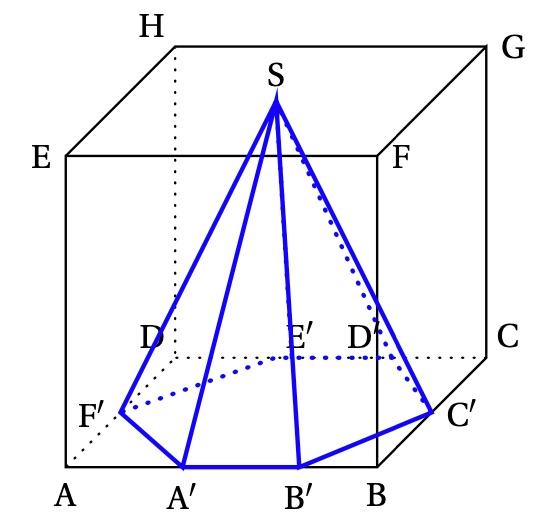
\includegraphics[width=0.5\linewidth]{img/bac_blanc_02.jpg}
  \caption{\label{} Représentation de la pyramide}
\end{figure}

\subsection*{Question 1}

On donne les coordonnées des points dans le repère \((A, \vec{\imath}, \vec{\jmath}, \vec{k})\) :
\begin{itemize}[noitemsep]
  \item Le sommet \(S\) est le centre de la face \(EFGH\). \\ 
  Sur l'axe des X ($\vec{\imath}$), il est donc entre le "x" de E et le "x" de F. Donc il se situe en 4 \\
  Sur l'axe des Y (qui correspond à $\vec{\jmath}$ et à l'alignement dans le sens $\overrightarrow{AD}$, il est entre E et H (et donc entre A et D en terme d'alignement sur l'axe des Y) : Donc en 4
  Sur l'axe des Z (qui correspond à $\vec{k}$ et à l'alignement dans le sens $\overrightarrow{AE}$), il est au niveau de E, c'est à dire à la hauteur 8 \\
  Donc les coordonnées sont $S = (4; 4; 8)$ \\
  Une autre méthode consiste à prendre la moyenne de chaque coordonées des points E, F, G, H puisque S est le centre du carré EFGH. Cela implique de déjà connaître les coordonées de E, de F, de G, et de H, mais la formule ressemblerait à cela : 
  
  \begin{align}
    S &= \left(\frac{0 + 8 + 8 + 0}{4}; \frac{8 + 8 + 0 + 0}{4}; \frac{8 + 8 + 8 + 8}{4}\right) \\
      &= (4; 4; 8).
    \end{align}
  
  \item Le point \(A'\) est à 3 cm de \(A\) sur \([AB]\). \([AB]\) correspond à l'axe des "abscisses" : il ne génère aucune avancée sur l'axe des "y", ni sur l'axe des "z". Et on sait que AA' = 3cm. Une unité de 1cm correspond à un incrément de 1 en termes de coordonées. Ses coordonnées sont :
  \[
  A' = (3; 0; 0).
  \]

  \item Pour B, on raisonne avec les longueurs : de AA', et de A'B'
  \begin{align*}
    AB' &= AA' + A'B' \\
    AB' &= 3 + 3 \\
    AB' = 6
    \end{align*} 
  \[
  B' = (6; 0; 0).
  \]

  \item Le point \(C'\) est le milieu de \([BC]\). On peut lire les coordonées, en sachant que C est avancé de 8 sur l'axe des abscisses, et de 4 sur l'axe des ordonnées. Une réponse sans justification était correcte. On pouvait aussi déterminé les coordonées de B et C : $B = (8;0;0)$ et $C = (8;8;0)$ puis appliquer la formule pour trouver les coordonées du milieu d'un côté : \\
  \[
    \left\{
    \begin{array}{l}
        x_{C'} = \frac{x_B + x_C}{2} \\
        y_{C'} = \frac{y_B + y_C}{2} \\
        z_{C'} = \frac{z_B + z_C}{2} \\
    \end{array}
    \right.
    \]
  
  Ses coordonnées sont :
  \[
  C' = \left(\frac{8 + 8}{2}; \frac{0 + 8}{2}; \frac{0 + 0}{2}\right) = (8; 4; 0).
  \]

  \item Le point \(E'\) : Le point E' est au même niveau que D sur l'axe des "y", il est donc à 8. En terme de "z", il est à 0 (il est au niveau du sol). La complexité réside dans sa valeur sur l'axe des x. On sait que DC = 8 (c'est une arête du cube). Et on sait que CD' = 3 et E'D' = 3.
  Donc
  \begin{align*}
    DE' + E'D' + D'C = 8 \\
    DE' + 3 + 3 = 8 \\
    DE' = 2
    \end{align*} 

  \[
  E' = (2; 8; 0).
  \]

  \item Le point \(F'\) est le milieu de \([AD]\). On applique le même raisonnement que pour les coordonées du point C. Les coordonnées de F' sont :
  \[
  F' = (0; 4; 0).
  \]
\end{itemize}

\textbf{Résultat final :} 
\begin{align*}
  S(4; 4; 8) \\
  A'(3; 0; 0) \\
  B'(6; 0; 0) \\
  C'(8; 4; 0) \\
  E'(2; 8; 0) \\
  F'(0; 4; 0)
\end{align*} 

\subsection*{Question 2}

\textbf{Calcul de la longueur du segment \([B'C']\) :} On utilise la formule de distance dans l’espace :
\[
d(B', C') = \sqrt{(x_C' - x_B')^2 + (y_C' - y_B')^2 + (z_C' - z_B')^2}.
\]
Substituons les coordonnées \(B'(6; 0; 0)\) et \(C'(8; 4; 0)\) :
\[
d(B', C') = \sqrt{(8 - 6)^2 + (4 - 0)^2 + (0 - 0)^2} = \sqrt{2^2 + 4^2} = \sqrt{4 + 16} = \sqrt{20} = 2 \times \sqrt{5}
\]
\vspace{1em}
\textbf{Conclusion : La longueur de \([B'C']\) est \(\sqrt{20} \approx 4.47\) cm} \\
\vspace{1em}
\textbf{Analyse du polygone de base : En terme de longueurs, on sait que A'B' = 3 cm. Et on vient de montrer que \(B'C' \approx 4.47\) cm. Les côtés adjacents \([A'B']\) et \([B'C']\) ont des longueurs différentes, donc le polygone A'B'C'D'E'F' ne peut pas être régulier}.  
\vspace{1em}

\subsection*{Question 3}

On peut aussi trouver la longueur de B'C' en utilisant le théorème de Pythagore dans le triangle \(B'BC'\) rectangle en B:
\[
B'C'^2 = B'B^2 + BC'^2.
\]

Pour calculer les longueurs de B'B et BC', il n'y a pas besoin d'utiliser les notions de coordonées. Un simple calcul de distances le long d'une droite suffit. : \\ 
Puisque A, A', B, B' sont alignés : 
\begin{align*}
  AA' + A'B' + B'B = 8 \\ 
  \text{or} \quad AA' = 3 \quad \text{et} \quad A'B' = 3 \\
  3 + 3 + B'B = 8 \\
  B'B = 2
\end{align*} 

\vspace{1em}
C' est au milieu de BC. La longueur de BC est 8. Donc on peut affirmer que BC' = 4.
\vspace{1em}
On substitue : \\ 
\[
  B'C'^2 = 2^2 + 4^2 = 4 + 20 \implies B'C' = \sqrt{20}
\]

\textbf{Conclusion :} La longueur trouvée est cohérente avec la question précédente.

\subsection*{Question 4}

Les vecteurs \(\overrightarrow{F'E'}\) et \(\overrightarrow{B'C'}\) sont donnés par leurs coordonnées :
\[
\overrightarrow{F'E'} = \begin{pmatrix}2 - 0 \\ 8 - 4 \\ 0 - 0\end{pmatrix} = \begin{pmatrix}2 \\ 4 \\ 0\end{pmatrix}, \quad 
\overrightarrow{B'C'} = \begin{pmatrix}8 - 6 \\ 4 - 0 \\ 0 - 0\end{pmatrix} = \begin{pmatrix}2 \\ 4 \\ 0\end{pmatrix}.
\]

Testons la colinéarité : il doit exister un réel \(\alpha\) tel que 
\[
\begin{pmatrix}2 \\ 4 \\ 0\end{pmatrix} = \alpha \cdot \begin{pmatrix}2 \\ 4 \\ 0\end{pmatrix}.
\]

L'éaglité fonctionne pour $\alpha = 1$. Plus précisément, les vecteurs sont totalement égaux : 

\[
  \overrightarrow{F'E'} = \overrightarrow{B'C'} = \begin{pmatrix}2 \\ 4 \\ 0\end{pmatrix}
\]

\textbf{\textcolor{blue}{Les vecteurs sont donc colinéaires et on peut en conclure que les droites \((F'E')\) et \((B'C')\) sont parallèles.}}

\section*{Exercice 2 [6 points] Les suites}

\begin{questions}
  \question[3] Soit la suite $(U_n)$ définie par :
  \[
  \left\{
  \begin{array}{l}
      U_{n+1} = U_n + 3, \\
      U_0 = 2.
  \end{array}
  \right.
  \]

  \begin{parts}
    \part[1] \textbf{Calcul des termes $U_1$, $U_4$, et $U_6$ :}

    Pour calculer chaque terme, nous devons partir de la définition de la suite et ajouter 3 au terme précédent. Voici les étapes détaillées :

    \begin{itemize}[noitemsep]
        \item Calcul de $U_1$ :
        \[
        U_1 = U_0 + 3 = 2 + 3 = 5.
        \]

        \item Calcul de $U_2$ :
        \[
        U_2 = U_1 + 3 = 5 + 3 = 8.
        \]

        \item Calcul de $U_3$ :
        \[
        U_3 = U_2 + 3 = 8 + 3 = 11.
        \]

        \item Calcul de $U_4$ :
        \[
        U_4 = U_3 + 3 = 11 + 3 = 14.
        \]

        \item Calcul de $U_5$ :
        \[
        U_5 = U_4 + 3 = 14 + 3 = 17.
        \]

        \item Calcul de $U_6$ :
        \[
        U_6 = U_5 + 3 = 17 + 3 = 20.
        \]
    \end{itemize}

    \textbf{Résultat :} Les termes demandés sont $U_1 = 5$, $U_4 = 14$, et $U_6 = 20$.

    \part[1] \textbf{Calcul de $U_{n+1} - U_n$ pour tout $n \in \mathbb{N}$ :}

    Par définition de la suite, nous savons que :
    \[
    U_{n+1} = U_n + 3.
    \]

    Ainsi :
    \[
    U_{n+1} - U_n = (U_n + 3) - U_n = 3.
    \]

    \textcolor{blue}{Conclusion importante :} La différence entre deux termes consécutifs de cette suite est toujours égale à 3.

    \part[0.5] \textbf{La suite est-elle croissante ou décroissante ?}

    Une suite est croissante si chaque terme est strictement supérieur au précédent. Ici, puisque $U_{n+1} - U_n = 3$ (un nombre positif), on peut conclure que la suite $(U_n)$ est croissante.

    \part[0.5] \textbf{Observation sur la nature de la suite dès la lecture de l'énoncé :}

    Une suite où l'on ajoute un nombre fixe (ici, $+3$) à chaque étape est appelée une \textcolor{red}{suite arithmétique}. Dès que l'on voit cette propriété dans l'énoncé, on sait que la suite sera croissante si la constante ajoutée est positive (ici $+3$) ou décroissante si elle est négative.
  \end{parts}

  \question[3] Soit la suite $(U_n)$ définie par :
  \[
  \left\{
  \begin{array}{l}
      U_{n+1} = U_n^2 + U_n + 2, \\
      U_0 = 1.
  \end{array}
  \right.
  \]

  \begin{parts}
      \part[1] \textbf{Calcul des termes $U_1$, $U_2$, et $U_3$ :}

      \begin{itemize}[noitemsep]
          \item Calcul de $U_1$ :
          \[
          U_1 = U_0^2 + U_0 + 2 = 1^2 + 1 + 2 = 1 + 1 + 2 = 4.
          \]

          \item Calcul de $U_2$ :
          \[
          U_2 = U_1^2 + U_1 + 2 = 4^2 + 4 + 2 = 16 + 4 + 2 = 22.
          \]

          \item Calcul de $U_3$ :
          \[
          U_3 = U_2^2 + U_2 + 2 = 22^2 + 22 + 2 = 484 + 22 + 2 = 508.
          \]
      \end{itemize}

      \textbf{Résultat :} Les termes demandés sont $U_1 = 4$, $U_2 = 22$, et $U_3 = 508$.

      \part[1] \textbf{Calcul de $U_{n+1} - U_n$ :}

      D'après l'expression de la suite :
      \[
      U_{n+1} - U_n = (U_n^2 + U_n + 2) - U_n = U_n^2 + 2.
      \]

      \textbf{Résultat :} $U_{n+1} - U_n = U_n^2 + 2$.

      \part[1] \textbf{Nature de la suite :}

      Le terme $U_{n+1} - U_n = U_n^2 + 2$ est toujours strictement positif, car $U_n^2 \geq 0$ pour tout $n$ (carré d'un nombre) et $+2$ est une constante positive. \textcolor{red}{Par conséquent, la suite $(U_n)$ est strictement croissante.}
  \end{parts}
\end{questions}

\section*{Correction de l'Exercice 2 [9 points] Les fonctions}

\begin{questions}
\question[2] Montrer que la fonction \(g(x) = x^2 - 4x - 12\) peut s'écrire sous la forme \((x-6)(x+2)\).

Pour factoriser \(g(x)\), on utilise une méthode simple :
\begin{itemize}[noitemsep]
    \item On cherche deux nombres dont :
        \begin{itemize}[noitemsep]
            \item le produit vaut \(-12\) (le terme constant) ;
            \item la somme vaut \(-4\) (le coefficient de \(x\)).
        \end{itemize}
    \item Ces deux nombres sont \(-6\) et \(2\) (car \(-6 \times 2 = -12\) et \(-6 + 2 = -4\)).
    \item On peut alors écrire :
    \[
    g(x) = x^2 - 4x - 12 = (x - 6)(x + 2).
    \]
\end{itemize}

\textbf{\textcolor{blue}{Conclusion :}} La fonction \(g(x)\) est bien factorisée sous la forme \((x - 6)(x + 2)\).

\question[0.5] En déduire les solutions de l'équation \(g(x) = 0\).

L'équation \(g(x) = 0\) revient à résoudre :
\[
(x - 6)(x + 2) = 0.
\]
Un produit est nul si et seulement si l'un des facteurs est nul. Donc :
\[
x - 6 = 0 \quad \text{ou} \quad x + 2 = 0.
\]
D'où :
\[
x = 6 \quad \text{ou} \quad x = -2.
\]

\textbf{\textcolor{blue}{Conclusion :}} Les solutions de \(g(x) = 0\) sont \(x = 6\) et \(x = -2\).

\question[0.5] Quelle est l'image de \(x = 1\) par la fonction \(g\) ?

On remplace \(x = 1\) dans l'expression de \(g(x)\) :
\[
g(1) = 1^2 - 4 \cdot 1 - 12.
\]
Effectuons les calculs étape par étape :
\begin{itemize}[noitemsep]
    \item \(1^2 = 1\) ;
    \item \(-4 \cdot 1 = -4\) ;
    \item \(1 - 4 = -3\) ;
    \item \(-3 - 12 = -15\).
\end{itemize}
Donc :
\[
g(1) = -15.
\]

\textbf{\textcolor{blue}{Conclusion :}} L'image de \(x = 1\) par la fonction \(g\) est \(-15\).

\question[1] Le point \(C(1 ; -12)\) appartient-il à la courbe représentative de \(g\) ? Qu'en est-il du point \(D(-2 ; 0)\) ? Justifier.

Un point \(P(a ; b)\) appartient à la courbe représentative de \(g\) si et seulement si \(g(a) = b\).

\begin{itemize}[noitemsep]
    \item Pour \(C(1 ; -12)\) :
    \[
    g(1) = -15 \quad \text{(calculé précédemment)}.
    \]
    Comme \(-15 \neq -12\), le point \(C\) n'appartient pas à la courbe.

    \item Pour \(D(-2 ; 0)\) :
    \[
    g(-2) = (-2)^2 - 4 \cdot (-2) - 12.
    \]
    Calculons étape par étape :
    \begin{itemize}[noitemsep]
        \item \((-2)^2 = 4\) ;
        \item \(-4 \cdot (-2) = 8\) ;
        \item \(4 + 8 = 12\) ;
        \item \(12 - 12 = 0\).
    \end{itemize}
    Donc \(g(-2) = 0\).

    Comme \(g(-2) = 0\), le point \(D(-2 ; 0)\) appartient à la courbe.
\end{itemize}

\textbf{\textcolor{blue}{Conclusion :}} \(C\) n'appartient pas à la courbe, mais \(D\) appartient à la courbe.

\question[2] Construire le tableau de signe de la fonction \(g\) sur le domaine de définition \(\mathcal{D} = \mathbb{R}\).

\textbf{Étape 1 :} Les solutions de \(g(x) = 0\) sont \(x = -2\) et \(x = 6\).

\textbf{Étape 2 :} \(g(x)\) change de signe aux valeurs \(x = -2\) et \(x = 6\). On teste les signes dans les intervalles \(\left]-\infty, -2\right[\), \(\left]-2, 6\right[\) et \(\left]6, +\infty\right[\) :
\begin{itemize}[noitemsep]
    \item Si \(x < -2\), les deux facteurs \((x - 6)\) et \((x + 2)\) sont négatifs, donc leur produit est positif.
    \item Si \(-2 < x < 6\), un facteur est positif et l'autre est négatif, donc leur produit est négatif.
    \item Si \(x > 6\), les deux facteurs sont positifs, donc leur produit est positif.
\end{itemize}

\textbf{Tableau de signe :}
\[
\begin{array}{|c|ccc|}
\hline
x & \; ]-\infty, -2[ \; & \; -2 \; & \; ]-2, 6[ \; & \; 6 \; & \; ]6, +\infty[ \; \\
\hline
g(x) & + & 0 & - & 0 & + \\
\hline
\end{array}
\]

\question[1] En déduire les solutions de l'inéquation \(g(x) \leq 0\).

D'après le tableau de signe, \(g(x) \leq 0\) pour \(x \in [-2 ; 6]\).

\textbf{\textcolor{blue}{Conclusion :}} Les solutions sont \(x \in [-2 ; 6]\).

\question[1] L'extremum (maximum ou minimum) d'un polynôme de degré 2 du type \(a x^2 + b x + c\) est atteint en \(x = -\frac{b}{2a}\). Quelles sont les coordonnées de l'extremum de \(g\) ?

Ici, \(a = 1\), \(b = -4\), donc :
\[
x = -\frac{-4}{2 \cdot 1} = \frac{4}{2} = 2.
\]
Pour trouver l'ordonnée correspondante :
\[
g(2) = 2^2 - 4 \cdot 2 - 12.
\]
Calculons étape par étape :
\begin{itemize}[noitemsep]
    \item \(2^2 = 4\) ;
    \item \(-4 \cdot 2 = -8\) ;
    \item \(4 - 8 = -4\) ;
    \item \(-4 - 12 = -16\).
\end{itemize}
Donc :
\[
g(2) = -16.
\]

\textbf{\textcolor{blue}{Conclusion :}} L'extremum est un minimum de coordonnées \((2 ; -16)\).

\question[1] En vous aidant du signe de \(a\) et grâce à la réponse à la question précédente, dresser le tableau de variation de \(g\).

\textbf{Le coefficient directeur \(a = 1\) est positif, donc la courbe a une forme de parabole ouverte vers le haut.}

\textbf{Tableau de variation :}
\[
\begin{array}{|c|c|c|c|}
\hline
x & \; ]-\infty, 2[ \; & \; 2 \; & \; ]2, +\infty[ \; \\
\hline
g(x) & \nearrow & -16 & \searrow \\
\hline
\end{array}
\]

\end{questions}

\end{document}
